\begin{center}
\begin{longtable}{ |l|l| } 
 \hline
 Attribute & Description\\ 
 \hline
 timestamp & time when first game starts\\ 
 \hline
 userId & ID of the user\\ 
 \hline
 nick & nickname chosen by the user\\ 
 \hline
 twitter & twitter handle of the user\\ 
 \hline
 dob & date of birth of the user\\ 
 \hline
 country & two letter country code of the user\\ 
 \hline
\caption{user.csv}
\end{longtable}
\end{center}

Data frame users is the first one (in this path) to have missing data. The data that is missing is in country and it is a small amount.
\begin{figure}[H]
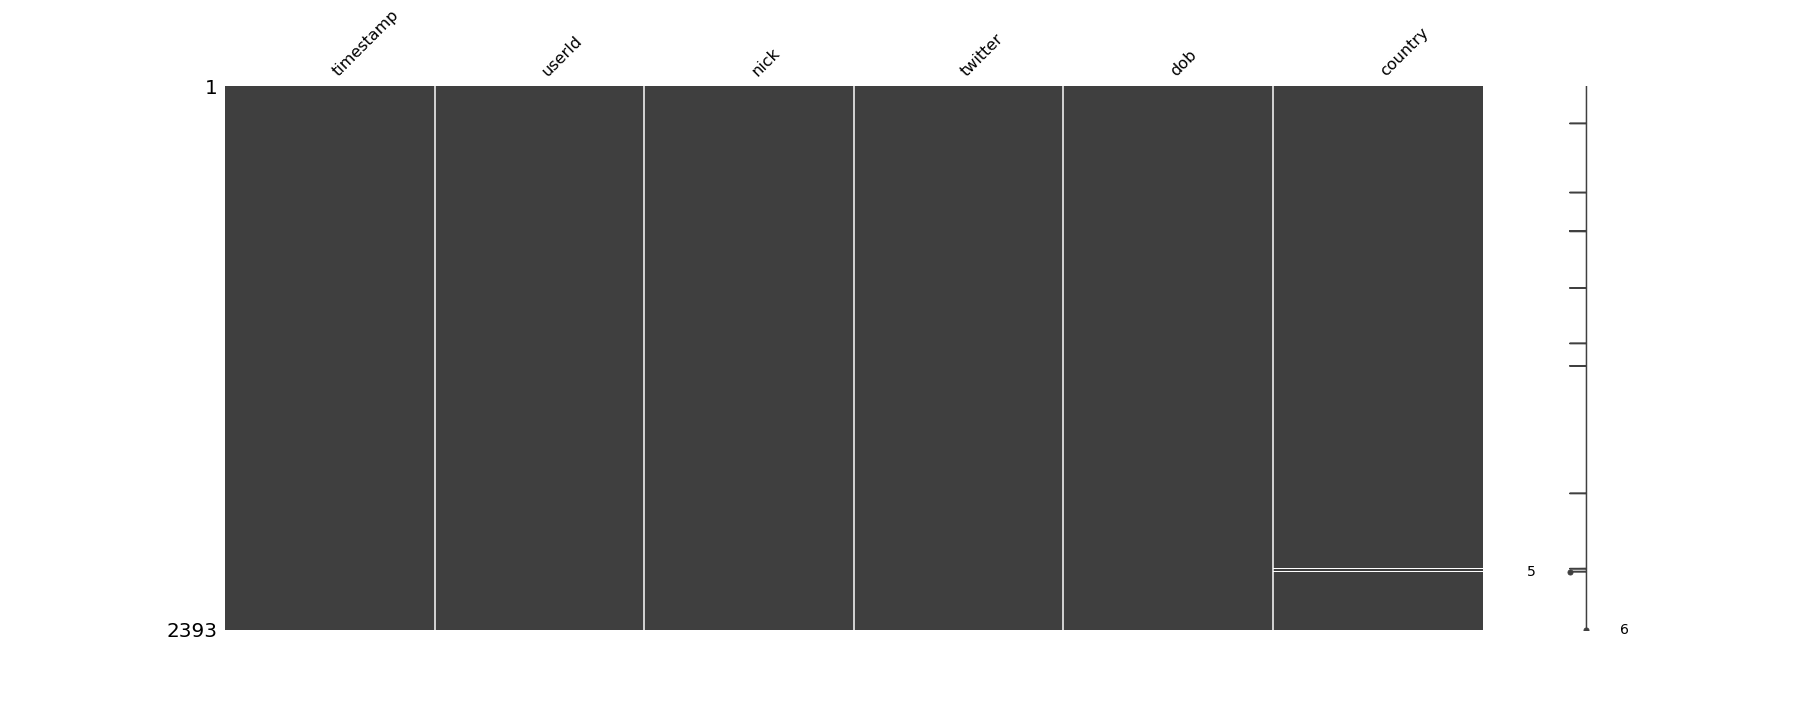
\includegraphics[scale=0.25]{img/Graphs/users/missingno_user.png}
\centering
\caption{missingno\_users}
\label{fig:missingno_user}
\end{figure}

The demographic of our users seem to be on the younger side. The majority of players seem to be born after 1970.
\begin{figure}[H]
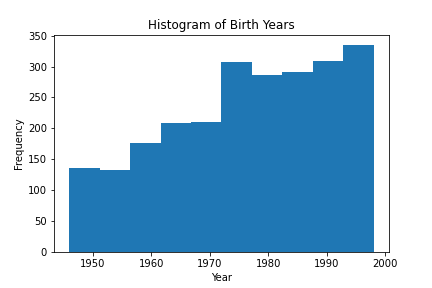
\includegraphics[scale=0.85]{img/Graphs/users/histogram_users.png}
\centering
\caption{histogram\_userSession}
\label{fig:histogram_users}
\end{figure}

\begin{landscape}
Geographically looking there seems to be players from all around the globe. This is good in terms of different markets and bad in terms of computational overhead (since we need computers in all of the regions for optimal performance).

    \begin{figure}[H]
        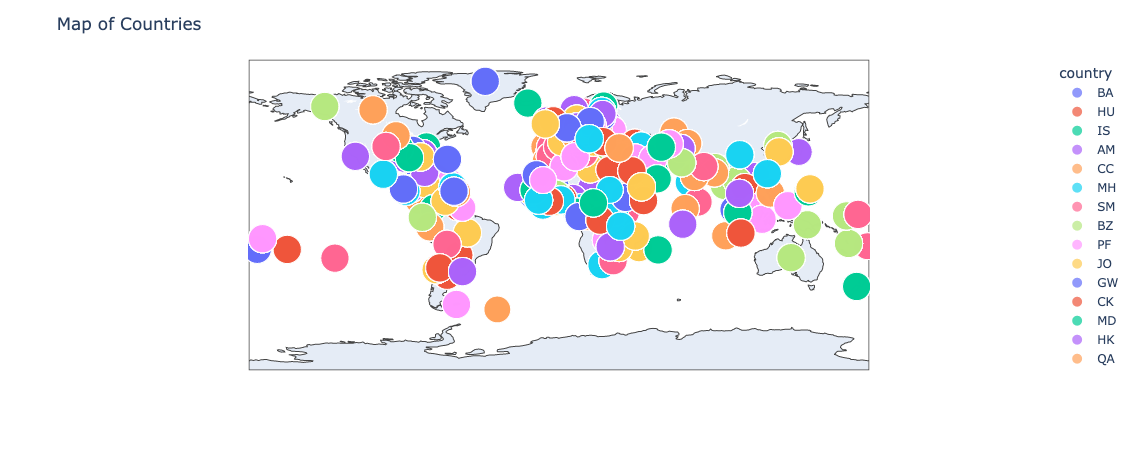
\includegraphics[scale=0.65]{img/Graphs/users/map.png}
        \centering
        \caption{map}
        \label{fig:map}
    \end{figure}
\end{landscape}